\begin{figure}[h]
	\centering
    \begin{tikzpicture}
    \node[inner sep=0pt] (pic) at (0,0)
    {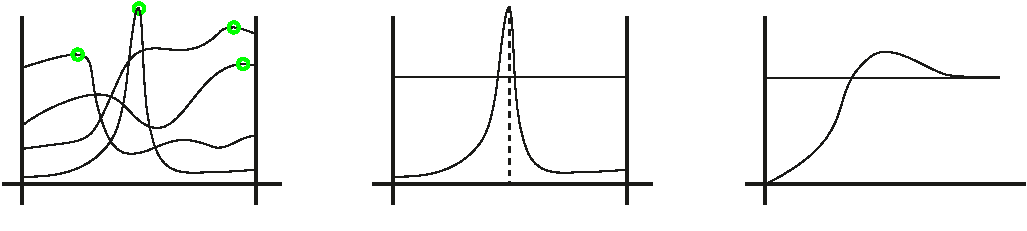
\includegraphics[width=15.0cm]{pictures/picture_3_4.pdf}};
    \draw [color=black](3,0.5) node[anchor=north west] {$ \delta $};
     \draw [color=black](0,-0.3) node[anchor=north west] {$ \theta $};
    \end{tikzpicture}
    \caption{1: zeleně suprema, nejmenší supremum je delta3 2: lepší je delta2, protože ač je riziko vysoké, jeho šance je velice malá - toto je nevýhoda minimaxní strategie 3: delta2 jen lehce překmitne delta1 a~pak se~k~němu blíží asymptoticky}
\end{figure}